\documentclass[12pt,letterpaper]{article}

% ---------- Packages ----------
\usepackage[letterpaper,margin=1in]{geometry}
\usepackage[T1]{fontenc}
\usepackage[utf8]{inputenc}
\usepackage{newtxtext,newtxmath} % Times-like font
\usepackage{microtype}
\usepackage{graphicx}
\usepackage{booktabs}
\usepackage{array}
\usepackage{tabularx}
\usepackage{enumitem}
\usepackage{titlesec}
\usepackage{xcolor}
\usepackage{hyperref}
\usepackage{fancyhdr}

% ---------- Colors (from Aspose export) ----------
\definecolor{brand}{rgb}{0.478431,0,0.235294}   % color_147093
\definecolor{accent}{rgb}{0.67451,0.078431,0.333333} % color_195788
\definecolor{textgray}{rgb}{0.2,0.2,0.2}        % color_80434
\definecolor{rulegray}{rgb}{0.866667,0.866667,0.866667} % color_249244

% ---------- Document styling ----------
\hypersetup{colorlinks=true,linkcolor=brand,urlcolor=accent,citecolor=brand}
\pagestyle{fancy}
\fancyhf{}
\lhead{}
\rhead{}
\lfoot{SE/CS 3RA3 — Fall}
\rfoot{\thepage}
\renewcommand{\headrulewidth}{0pt}
\renewcommand{\footrulewidth}{0.4pt}

\titleformat{\section}{\Large\bfseries\color{brand}}{\thesection}{0.75em}{}
\titleformat{\subsection}{\large\bfseries\color{brand}}{\thesubsection}{0.75em}{}
\titleformat{\subsubsection}{\normalsize\bfseries\color{brand}}{\thesubsubsection}{0.75em}{}

\setlist[itemize]{topsep=4pt,itemsep=2pt,parsep=0pt}
\setlist[enumerate]{topsep=4pt,itemsep=2pt,parsep=0pt}

% ---------- Title page ----------
\makeatletter
\def\@maketitle{%
  \begin{center}
    \vspace*{1.5cm}
    {\Huge\bfseries\color{brand} Our Awesome Project\par}
    \vspace{0.35cm}
    {\Large\itshape\color{accent} Requirements Standard Plan\par}
    \vspace{0.9cm}
    {\large Saad Salman, Author 2, Author 3\par}
    \vspace{0.25cm}
    {\normalsize Version 1, 2025-09-22\par}
    \vspace{1.5cm}
  \end{center}
}
\makeatother
\title{}
\author{}
\date{}

\begin{document}
\maketitle
\thispagestyle{empty}
\clearpage

\tableofcontents
\clearpage

% ---------- Academic Integrity Disclaimer ----------
\section*{Academic Integrity Disclaimer}
\addcontentsline{toc}{section}{Academic Integrity Disclaimer}
We would like to acknowledge that as dedicated students of McMaster University, we have thoroughly read and comprehended the Academic Integrity Policy published by the university. We are committed to upholding the principles of academic honesty and integrity in all aspects of our educational journey. We understand the importance of acknowledging the work and ideas of others, and we pledge to ensure that all our academic endeavors are conducted with the utmost originality and compliance with the university’s policy.

We affirm that the content presented in this document is entirely our own, and any external sources used have been appropriately cited and referenced.

\medskip
\noindent\textbf{Saad Salman} \\
As I submit my work, I, Saad Salman, take full responsibility for the integrity of my work and promise to avoid any form of plagiarism, cheating, or dishonest behavior. This acknowledgment serves as a testament to my dedication to academic excellence and the fostering of a trustworthy academic community at McMaster University.

\medskip
\noindent\textbf{Author 2} \\
As I submit my work, I, Author 2, take full responsibility for the integrity of my work and promise to avoid any form of plagiarism, cheating, or dishonest behavior. This acknowledgment serves as a testament to my dedication to academic excellence and the fostering of a trustworthy academic community at McMaster University.

\medskip
\noindent\textbf{Author 3} \\
As I submit my work, I, Author 3, take full responsibility for the integrity of my work and promise to avoid any form of plagiarism, cheating, or dishonest behavior. This acknowledgment serves as a testament to my dedication to academic excellence and the fostering of a trustworthy academic community at McMaster University.

\medskip
\noindent\textit{Policy:} \url{https://secretariat.mcmaster.ca/app/uploads/Academic-Integrity-Policy-1-1.pdf}

\clearpage

% ---------- Control Information ----------
\section{Control Information}
\begin{table}[h!]\centering
\caption*{Versioning and Delivery}
\renewcommand{\arraystretch}{1.2}
\begin{tabularx}{\textwidth}{@{}l l l l l l@{}}
\toprule
\textbf{Version} & \textbf{Delivery Deadline} & \textbf{Delivered} & \textbf{Feedback Received} & \textbf{Integrated} & \textbf{Notes} \\
\midrule
V1 & & & & & \\
V2 & & & & & \\
V3 & & & & & \\
\bottomrule
\end{tabularx}
\end{table}

\medskip
\noindent\textbf{Saad Salman} \\
Here is a quick biography of Saad Salman. You can contact them at \href{mailto:salmam12@mcmaster.ca}{salmam12@mcmaster.ca}.

\medskip
\noindent\textbf{Author 2} \\
Here is a quick biography of Author 2. You can contact them at \href{mailto:a2@mcmaster.ca}{a2@mcmaster.ca}.

\medskip
\noindent\textbf{Author 3} \\
Here is a quick biography of Author 3. You can contact them at \href{mailto:a3@mcmaster.ca}{a3@mcmaster.ca}.

\clearpage

% ---------- (G) Goals ----------
\section{(G) Goals}
\subsection*{Reading Guide}
Goals are ``needs of the target organization, which the system will address''. While the development team is the principal user of the other books, the Goals book addresses a wider audience: essentially, all stakeholders \cite{meyer2022}. It must contain enough information to provide---if read just by itself---a general sketch of the entire project. To this effect, chapter G.3 presents a short overview of the system and G.1 will typically include some key properties of the environment. As it addresses a wide readership, it should be clear and minimize the use of specialized technical terms. Together, G.1, G.2 and G.3 describe the rationale for the project. It is important to state these justifications explicitly. Typically, they are well understood at the start of the project, but management and priorities can change \cite{meyer2022}.

\subsection*{Control Information}
\begin{table}[h!]\centering
\caption*{Table 1. Our Awesome Project --- Versioning Information --- Goal Book}
\renewcommand{\arraystretch}{1.1}
\begin{tabularx}{\textwidth}{@{}l l l l l l@{}}
\toprule
\textbf{Section} & \textbf{Version} & \textbf{Lead} & \textbf{Delivered on} & \textbf{Reviewer} & \textbf{Approved on} \\
\midrule
G.1 & M1 & SS & Sept-21-2025 & SP & Sept-22-2025 \\
G.2 & M1 & SS & Sept-21-2025 & SP & Sept-22-2025 \\
G.3 & & & & & \\
G.4 & & & & & \\
G.5 & & & & & \\
G.6 & & & & & \\
G.7 & & & & & \\
\bottomrule
\end{tabularx}
\end{table}

\subsection{(G.1) Context and Overall Objectives}
High-level view of the project: organizational context and reason for building a system. It explains why the project is needed, recalls the business context, and presents the general business objectives \cite{meyer2022}.

New university students trying to make connections with each other can often find it difficult due to the limited interactions they have outside of their program. \textit{HammerCorp Inc.} will address this by developing a web and mobile app called \textbf{ACME Connect}, which connects students based on similar interests or experiences, as well as student clubs or institutional activities. It aims to improve the overall university experience by creating a tightly-knit student community where integration of official activities happens at the student level. With safety as a primary goal, this project plans to be available to universities across North America, with a pilot program starting at McMaster University.

\subsection{(G.2) Current Situation}
Current state of processes to be addressed by the project and the resulting system. It describes the current situation upon which the system is expected to improve \cite{meyer2022}.

At the moment, students are limited to in-person connections within their program or at Welcome Week events, which are often not sufficient for engagement and networking. Residence and international students may feel disconnected in a new place. Student clubs and associations also find it difficult to engage potential members. Although there are in-person events for new students and club booths around campus, those are temporary pop-ups and may not reach everyone. There is no central place for everyone to connect outside those events. Discord servers exist; however, they are often not institutionally based, which can compromise safety and allow complete strangers not affiliated with the school. Looking at these challenges, \textbf{ACME Connect} plans to address them and create a safe environment for students and institutions to foster lasting relationships throughout the university journey.

\subsection{(G.3) Expected Benefits}
New processes, or improvements to existing processes, made possible by the project’s results. It presents the business benefits expected from successful execution of the project. This chapter is the core of the Goals book, describing what the organization expects from the system \cite{meyer2022}.

\textit{Nothing available at this point.}

\subsection{(G.4) Functionality Overview}
Overview of the functions (behavior) of the system. Principal properties only (details are in the System book). A capsule version of book S that enables readers to get a quick grasp of what the system will do \cite{meyer2022}.

\textit{Nothing available at this point.}

\subsection{(G.5) High-level Usage Scenarios}
Fundamental usage paths through the system, stated in user terms and independent of the system’s structure. Detailed usage scenarios appear in the System book (S.4) \cite{meyer2022}.

\begin{center}
\fbox{\parbox{0.7\linewidth}{\centering \emph{(High level use case diagram placeholder)}}}
\end{center}

\textit{Nothing available at this point.}

\subsection{(G.6) Limitations and Exclusions}
Aspects that the system need not address; scoping the requirements. (Risks and obstacles belong to P.6.) \cite{meyer2022}.

\textit{Nothing available at this point.}

\subsection{(G.7) Stakeholders and Requirements Sources}
Stakeholder categories that can affect or be affected by the project, and other sources of requirements information \cite{meyer2022}.

\textit{Nothing available at this point.}

\clearpage

% ---------- (E) Environment ----------
\section{(E) Environment}
The Environment book describes the application domain and external context (physical or virtual) in which the system will operate \cite{meyer2022}.

\subsection*{Control Information}
\begin{table}[h!]\centering
\caption*{Table 2. Our Awesome Project --- Versioning Information --- Environment Book}
\renewcommand{\arraystretch}{1.1}
\begin{tabularx}{\textwidth}{@{}l l l l l@{}}
\toprule
\textbf{Section} & \textbf{Version} & \textbf{Lead} & \textbf{Delivered} & \textbf{Reviewer / Approved} \\
\midrule
E.1 & & & & \\
E.2 & & & & \\
E.3 & & & & \\
E.4 & & & & \\
E.5 & & & & \\
E.6 & & & & \\
\bottomrule
\end{tabularx}
\end{table}

\subsection{(E.1) Glossary}
Clear and precise definitions of all vocabulary specific to the application domain \cite{meyer2022}.

\textit{Nothing available at this point.}

\subsection{(E.2) Components}
List of environment elements that may affect or be affected by the system and project, including other systems for interfacing \cite{meyer2022}.

\textit{Nothing available at this point.}

\subsection{(E.3) Constraints}
Obligations and limits imposed by the environment (business rules, physical laws, engineering decisions) \cite{meyer2022}.

\textit{Nothing available at this point.}

\subsection{(E.4) Assumptions}
Environment properties assumed to hold to facilitate the system’s construction \cite{meyer2022}.

\textit{Nothing available at this point.}

\subsection{(E.5) Effects}
Elements and properties of the environment that the system will affect \cite{meyer2022}. Effects of the application include:
\begin{itemize}
  \item \textbf{Improved student belonging and wellbeing:} The application fosters safe and supportive environments that help students feel less isolated and more connected during the transition to university.
  \item \textbf{Increased participation in campus life:} By lowering barriers to joining clubs, events, and residence activities, the app encourages higher engagement with student associations and university-led initiatives.
  \item \textbf{Enhanced student retention and success:} With better access to support networks and resources, students are less likely to drop out due to isolation or lack of integration.
\end{itemize}

\subsection{(E.6) Invariants}
Environment properties that the system’s operation must preserve \cite{meyer2022}.

\textit{Nothing available at this point.}

\clearpage

% ---------- (S) System ----------
\section{(S) System}
The System book refines the Goals book by focusing on more detailed requirements.

\subsection{(S.1) Components}
Hitchly is composed of 6 main components that collectively provide the necessary functionality required for the application. \\

\noindent \textbf{Matchmaking Engine:} The matchmaking engine is responsible for matching riders with drivers based on schedules/timetables, departure times, routes and locations, and other user preferences. 
It interfaces with the scheduling system to ensure rides can be matched, whether it be one-time or recurring. It will optimize for cost, convenience, and schedule alignment. \\

\noindent \textbf{Scheduling and Booking Manager:} Allows users to upload their schedules to inform about their availability to facilitate matchmaking. It also ensures booked rides are stored, updated, or cancelled as per defined policies.  \\

\noindent \textbf{Safety and Verification Module:} This module provides secure login through McMaster email authentication. This ensures that only verified students and staff at McMaster may use the system, providing reassurance and safety for users and a sense of community. \\

\noindent \textbf{Payment and Cost Sharing System:} This system automatically calculates the cost of the ride for each rider based on the distance, number of passengers, gas, and parking costs. It manages in-app payment transactions and a transparent fee breakdown. \\

\noindent \textbf{User Profile Manager:} Stores user details such as a profile picture, bio, ratings, preferences, and more. Allows other users to view a profile when matching with each other to see information about them, as well as reliability metrics such as completed rides, any strikes, and more. \\

\noindent \textbf{Rating and Reputation System:} Tracks the attendance, punctuality, and safety related behaviour of drivers and riders. Issues strikes and penalties as needed, and integrates with the user profile manager to display user ratings and history. \\
\vspace{1em}

\begin{samepage}
\noindent The following diagram shows how these components interact and communicate when the application is being used.
\begin{figure}[!h]
  \centering
  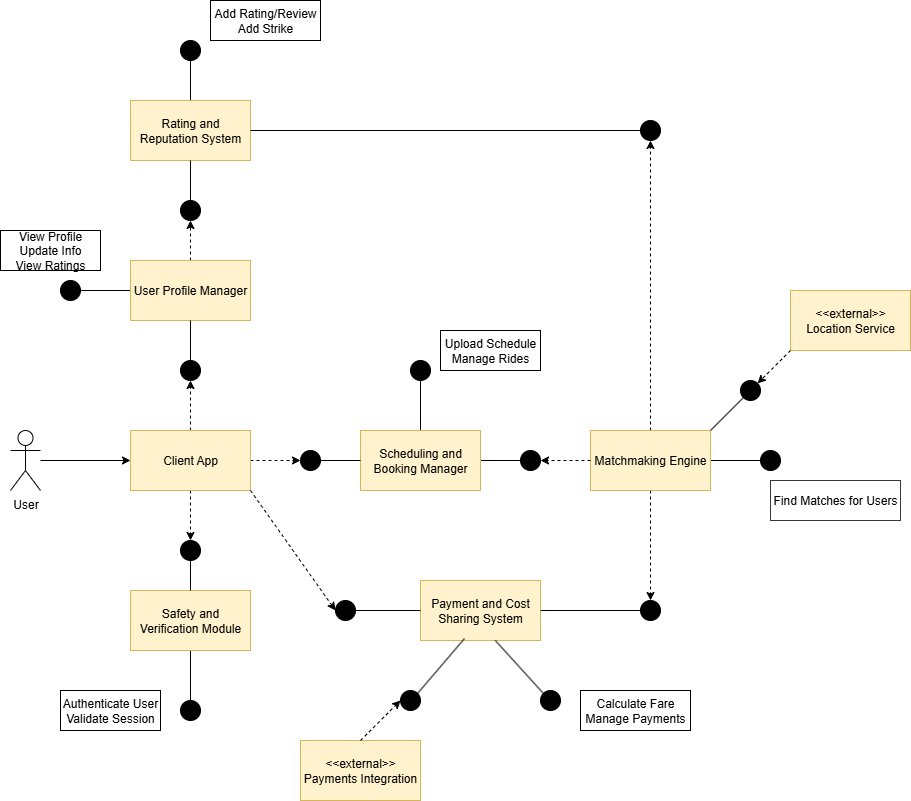
\includegraphics[width=0.9\textwidth]{component_diagram.png}
  \caption{Hitchly Component Diagram.}
\end{figure}
\end{samepage}
\clearpage

\subsection{(S.2) Functionality}
The bulk of the System book: functional and non-functional behaviors \cite{meyer2022}.

\textit{Nothing available at this point.}

\subsection{(S.3) Interfaces}
How the system makes S.2 functionality available to the rest of the world (UIs and APIs) \cite{meyer2022}.

\textit{Nothing available at this point.}

\subsection{(S.4) Detailed Usage Scenarios}
User stories and examples of interaction between users/environment and the system \cite{meyer2022}.

\textit{Nothing available at this point.}

\subsection{(S.5) Prioritization}
Classification of behaviors, interfaces, and scenarios by criticality \cite{meyer2022}.

\textit{Nothing available at this point.}

\subsection{(S.6) Verification and Acceptance Criteria}
Conditions under which an implementation will be deemed satisfactory; V\&V levels \cite{meyer2022}.

\textit{Nothing available at this point.}

\clearpage

% ---------- (P) Project ----------
\section{(P) Project}

\subsection{(P.1) Roles and Personnel}
Main responsibilities, required staff, and qualifications \cite{meyer2022}.

\textit{Nothing available at this point.}

\subsection{(P.2) Imposed Technical Choices}
A priori choices binding the project to specific tools, hardware, languages or other technical parameters \cite{meyer2022}.

\textit{Nothing available at this point.}

\subsection{(P.3) Schedule and Milestones}
List of tasks to be carried out and their scheduling \cite{meyer2022}.

\textit{Nothing available at this point.}

\subsection{(P.4) Tasks and Deliverables}
Details of individual tasks and expected outcomes, associated with milestone dates \cite{meyer2022}.

\textit{Nothing available at this point.}

\subsection{(P.5) Required Technology Elements}
External systems, hardware and software expected to be necessary for building the system \cite{meyer2022}.

\textit{Nothing available at this point.}

\subsection{(P.6) Risk and Mitigation Analysis}
Potential obstacles to meeting the schedule and measures for adapting the plan \cite{meyer2022}.

\textit{Nothing available at this point.}

\subsection{(P.7) Requirements Process and Report}
Initially: description of the requirements process; later: report on its steps \cite{meyer2022}.

\textit{Nothing available at this point.}

\clearpage

% ---------- References ----------
\begin{thebibliography}{9}
\bibitem{meyer2022} Bertrand Meyer. \textit{Handbook of Requirements and Business Analysis}. Springer, 2022.
\bibitem{sommerville1997} Ian Sommerville and Peter Sawyer. \textit{Requirements Engineering: A Good Practice Guide}. Wiley, 1997.
\end{thebibliography}

\end{document}